\subsection{Introduction}
Following the initial wave simulator developed with OpenMP, this second assignment extends the application to execute multiple concurrent simulations on an HPC system using a hybrid MPI and OpenMP programming model. The goal is to study multi-wave interaction and interference dynamics under different physical conditions. While OpenMP continues to handle data parallelism by accelerating the 2D stencil computations across local CPU cores, MPI is introduced to manage task parallelism. Specifically, the system executes three distinct simulation scenarios simultaneously within a single execution run:
\begin{itemize}
\item \textbf{Simulation 1 (Rank 0):} Reproduces the baseline single-wave scenario initiated by a single central impulse at coordinates $(M/2, M/2)$ at $t = 0$.
\item \textbf{Simulation 2 (Rank 1):} Models wave superposition and interference phenomena by initiating two simultaneous impulses at different spatial locations at $t = 0$.
\item \textbf{Simulation 3 (Rank 2):} Introduces time-delayed interference dynamics by generating a second impulse at a spatial location after a predetermined time-shift ($t = t_{start}$).
\end{itemize}
By decoupling these independent workloads across separate MPI processes, the hybrid architecture maximizes computational throughput without requiring inter-process communication during the time-stepping loop.

\subsection{Implementation}

Building upon the code developed in Assignment 1, the implementation extends the simulator to handle multiple concurrent runs. The core numerical scheme for the time-stepping propagation and the mapping function converting field values into grayscale images (\textbf{write\_matrix}) remain identical to the first version, ensuring consistency in wave physics and visualization.

The execution starts by initializing the MPI environment with \textbf{MPI\_Init}, retrieving the total number of processes with \textbf{MPI\_Comm\_size}, and identifying the rank ID of each process with \textbf{MPI\_Comm\_rank}. To run the three required simulations simultaneously, the program verifies that at least 3 processes are allocated. Task parallelism is managed through conditional branching based on the process rank, where each rank specifies its scenario parameters before calling a dedicated \textbf{run\_simulation} function that encapsulates the core time-stepping loop.

While data parallelism within each process is handled by OpenMP, the execution incorporates rank-specific logic. Thread synchronization constructs, such as the \textbf{pragma omp single} directive, are carefully utilized within the time loop to safely manage tasks that must be executed by a single thread—such as array pointer swapping, injecting the delayed impulse, and saving frames—preventing race conditions without halting the entire team of threads unnecessarily.
\subsection{Test and Optimization}
A fundamental optimization in this hybrid architecture concerns memory management. Each MPI process independently allocates memory for its local grid arrays (\textbf{u\_past}, \textbf{u}, and \textbf{u\_fut}) utilizing a custom \textbf{matrix\_alloc} function. Although there is no inter-process communication between the MPI ranks in this specific decoupled setup, contiguous memory allocation remains crucial for the local OpenMP threads. It maximizes spatial locality and hardware prefetching efficiency, ensuring that the CPU cache is utilized optimally during the 2D stencil computations. This approach significantly helps to mitigate the heavy contention on the main RAM caused by the three concurrent processes. 

A second crucial aspect is minimizing thread synchronization overhead. While data parallelism is handled by OpenMP, tasks that must be executed by a single thread, such as array pointer swapping and saving frames, require synchronization constructs like the \textbf{pragma omp single} directive. To optimize this, the injection of the time-delayed impulse for Simulation 3 in the rank 2 was carefully structured. Instead of placing the conditional check inside a synchronized block, the evaluation (\textbf{if (rank == 2 \&\& t == n\_start)}) is placed strictly \textit{outside} the \textbf{pragma omp single} directive. This architectural choice ensures that the threads only encounter the synchronization barrier at the exact time step when the impulse must be applied. During all other time steps, and for all other simulation ranks, the threads completely bypass the barrier, preventing race conditions without halting the entire team of threads unnecessarily and drastically reducing idle times. 

Following these code optimizations, the execution times of the three ranks were profiled, executed with 8 OpenMP threads per rank. As expected from a well-balanced workload, the execution times show no significant variation among the three processes, demonstrating excellent load balancing despite the ranks having different initial conditions and logic branches. However, when comparing these results to the baseline times from Assignment 1, a severe performance degradation is observed as the matrix size ($M$) increases.
\begin{figure}[htbp]
    \centering
    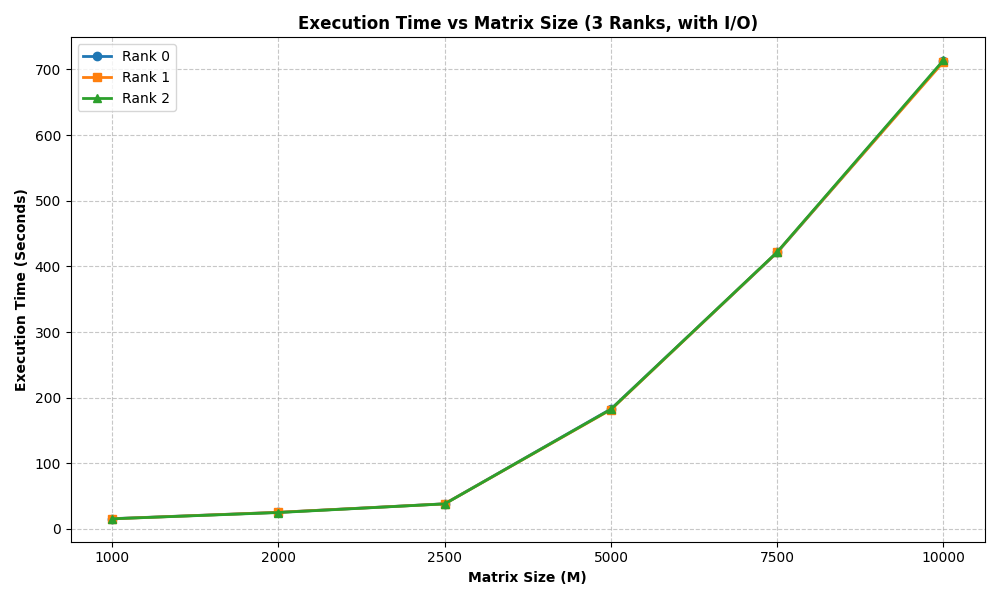
\includegraphics[width=0.8\textwidth]{../Giro_part/Esercizio_2/Grafici/Grafico_tempi_variandoM_conIO.png}
    \caption{Execution Time vs Matrix Size.}
    \label{fig:graph_1}
\end{figure}

This massive slowdown is not caused by the computational complexity of the hybrid setup, but by an Input/Output (I/O) bottleneck. The simultaneous memory access and disk-writing operations to the shared file system by all three MPI processes, each attempting to format and save \textbf{.pgm} frames concurrently, create heavy hardware contention. This I/O saturation stalls the CPU threads, drastically inflating the overall execution time for all processes involved.

To isolate and evaluate the purely computational performance of the hybrid architecture, the disk-writing operations (I/O) were temporarily disabled. The profiling tests were then re-executed, varying the matrix size ($M$) while maintaining the configuration of 8 OpenMP threads per MPI task. 

In the first optimization phase, all three ranks (totaling 24 threads) were deliberately confined to a single CPU socket to evaluate shared memory contention. 

\begin{figure}[htbp]
    \centering
    % Sostituisci il percorso qui sotto con il nome del PRIMO grafico combo
    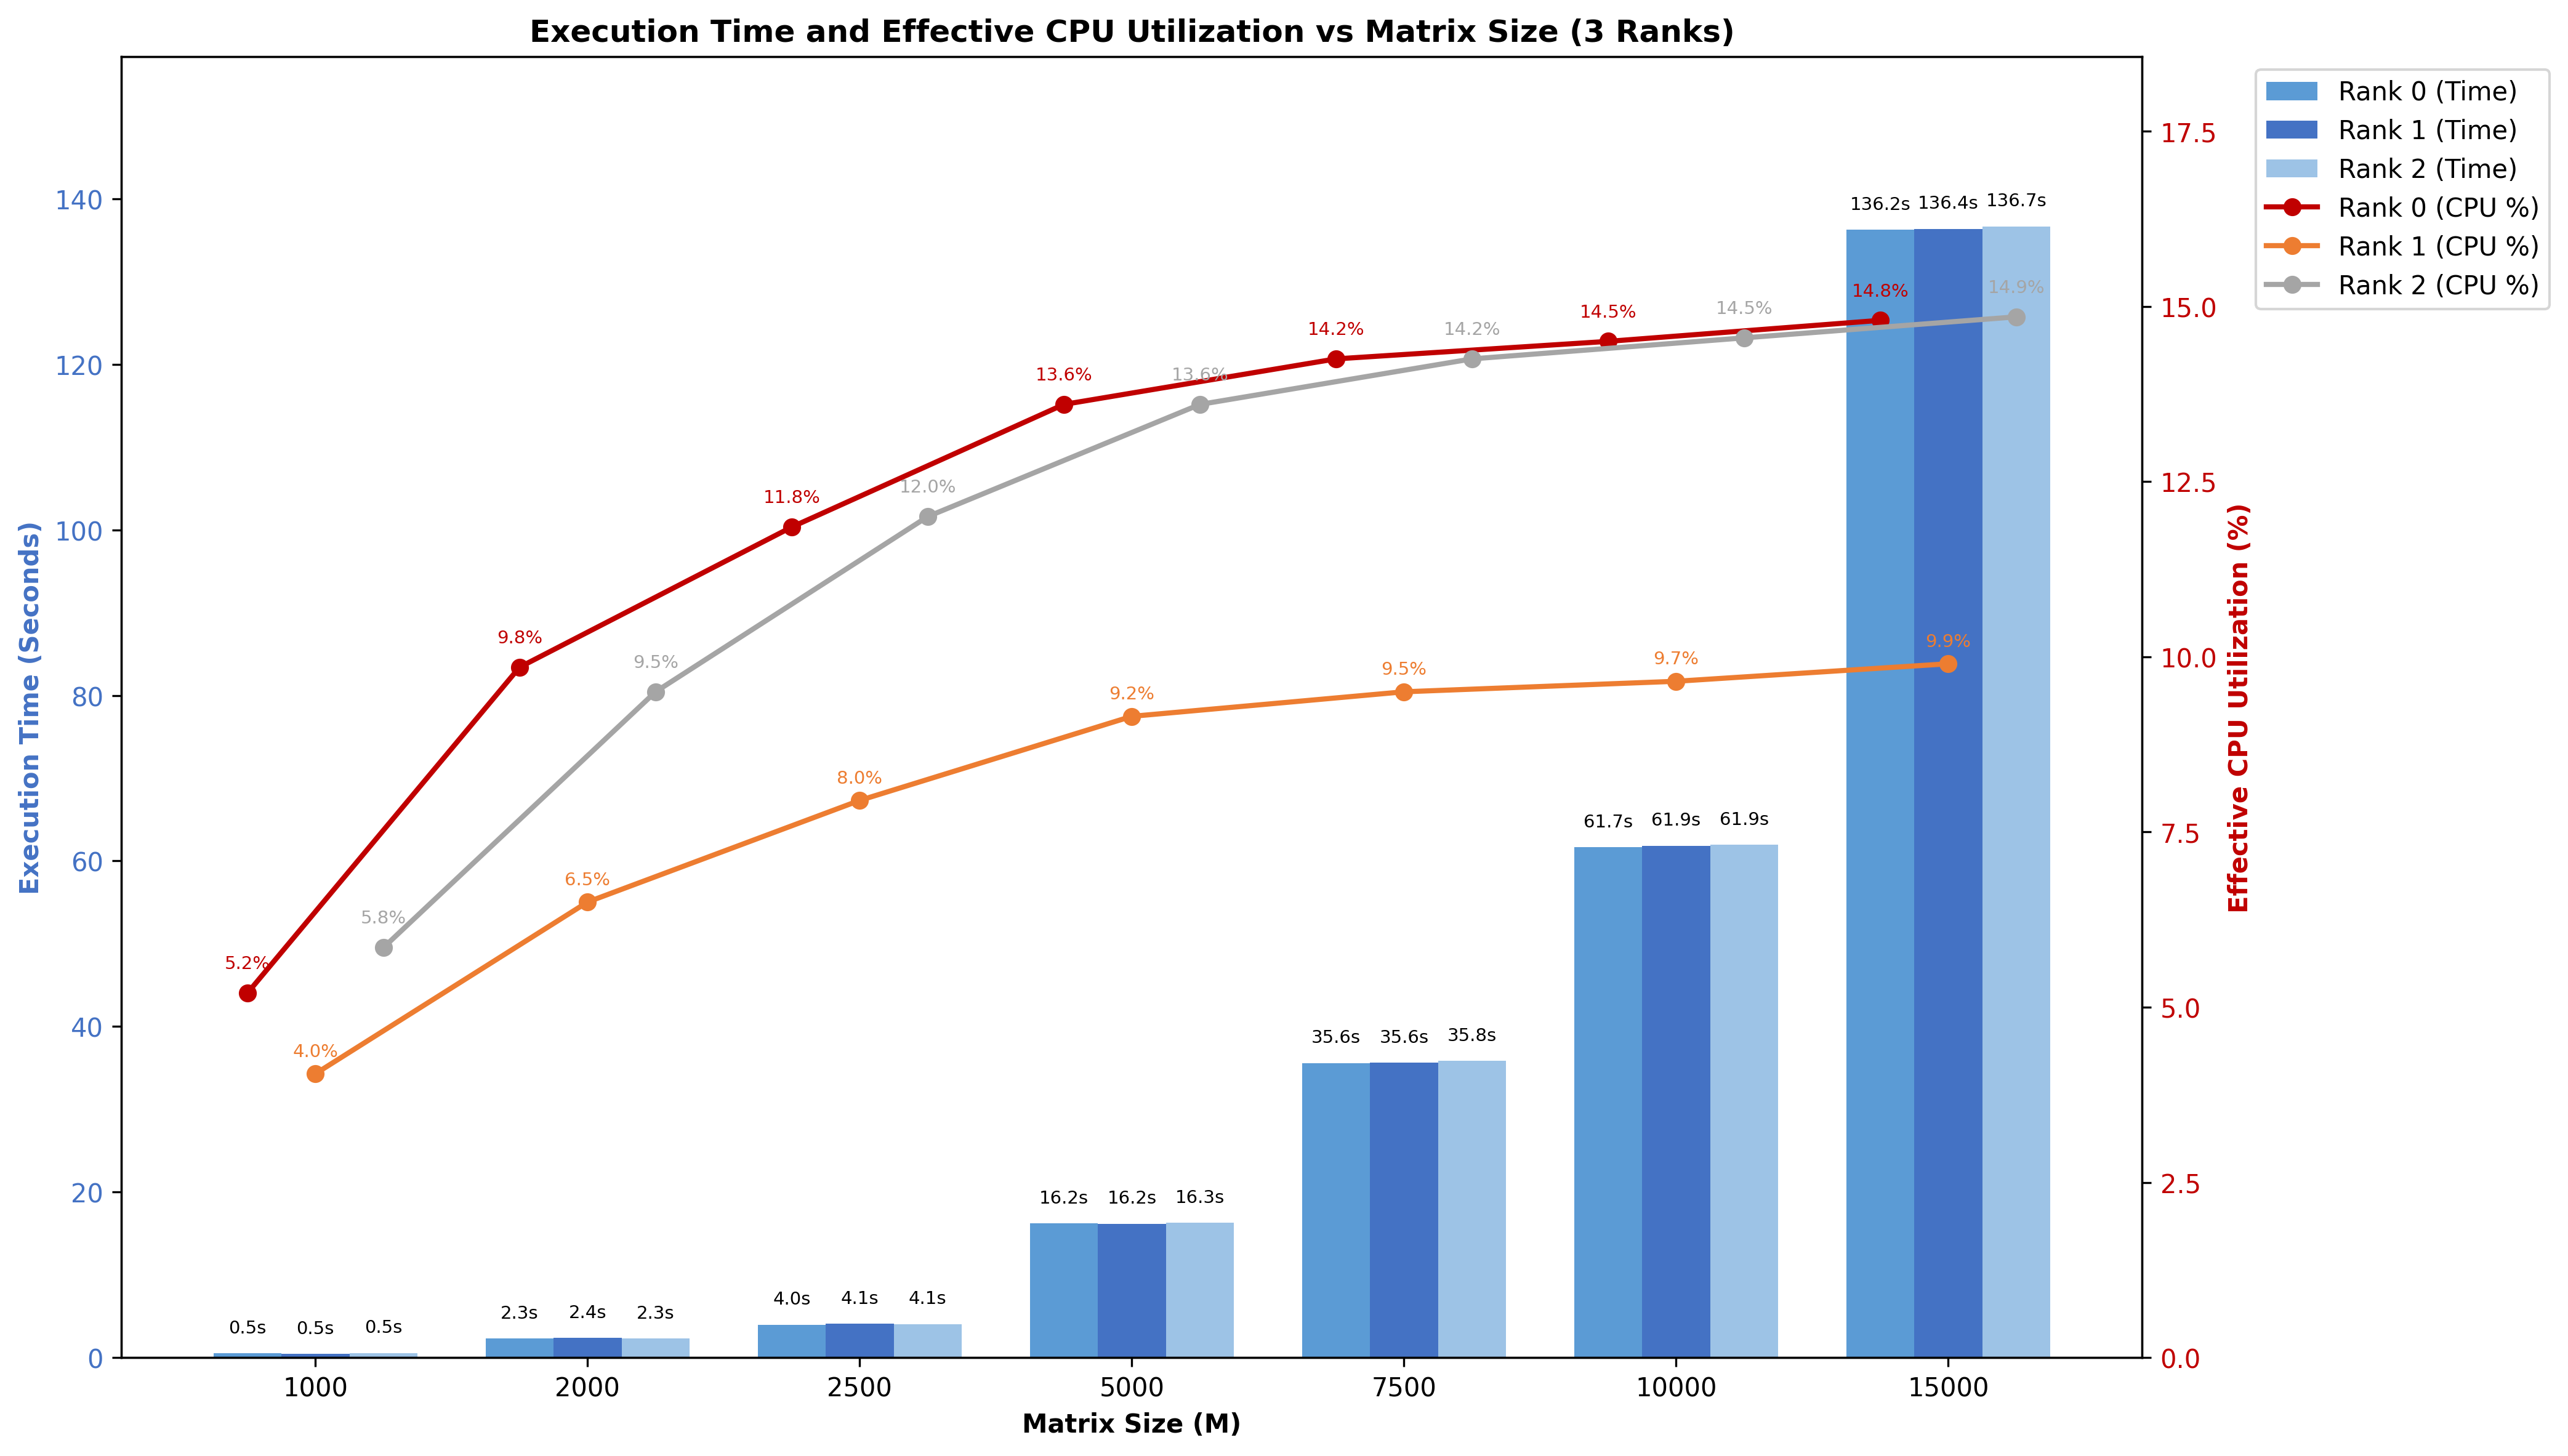
\includegraphics[width=0.9\textwidth]{../Giro_part/Esercizio_2/Grafici/combo_bars_lines_1socket.png}
    \caption{Execution Time and Effective CPU Utilization vs Matrix Size (3 Ranks confined to a single socket without strict pinning).}
    \label{fig:graph_single_socket}
\end{figure}

As illustrated in Figure \ref{fig:graph_single_socket}, eliminating the I/O bottleneck yields a drastic reduction in execution times, dropping from over 700 seconds to approximately 136 seconds for $M=15000$. This result is closely aligned with the 123 seconds observed in the Assignment 1 baseline, which, notably, was executed using only a single process. However, the Intel VTune profiling reveals a significant hardware-level anomaly: the Effective CPU Utilization is highly asymmetric. Rank 1 exhibits a drastically lower efficiency percentage compared to Ranks 0 and 2. Since the three processes execute the exact same computational volume, this discrepancy is not due to algorithmic imbalance. 

Instead, because the 24 threads were executed within a single socket without strict hardware pinning, the Linux operating system attempted to optimize execution management by occasionally migrating computations from heavily utilized cores to colder ones. When a thread wakes up on a newly assigned core and attempts to compute the 2D stencil, it experiences a "cache miss" \cite{sanchez_cache}. Since each physical core relies on its own local level of cache, the required grid data is no longer immediately available. The processor is therefore forced to fetch the data all the way from the main RAM. This memory access operation is extremely slow and causes a memory stall, effectively freezing the CPU while it waits for the data to arrive. This phenomenon predominantly affected the threads of Rank 1, and these continuous RAM access stalls are the exact reason why its Effective CPU Utilization is severely degraded compared to the other two processes.

To validate this memory contention hypothesis, a second profiling test was conducted by physically distributing the ranks across the node's Non-Uniform Memory Access (NUMA) architecture. Rank 0 and Rank 2 were strictly pinned to Socket 0, while Rank 1 was granted exclusive access to Socket 1.

\begin{figure}[htbp]
    \centering
    % Sostituisci il percorso qui sotto con il nome del SECONDO grafico combo (quello sfalsato)
    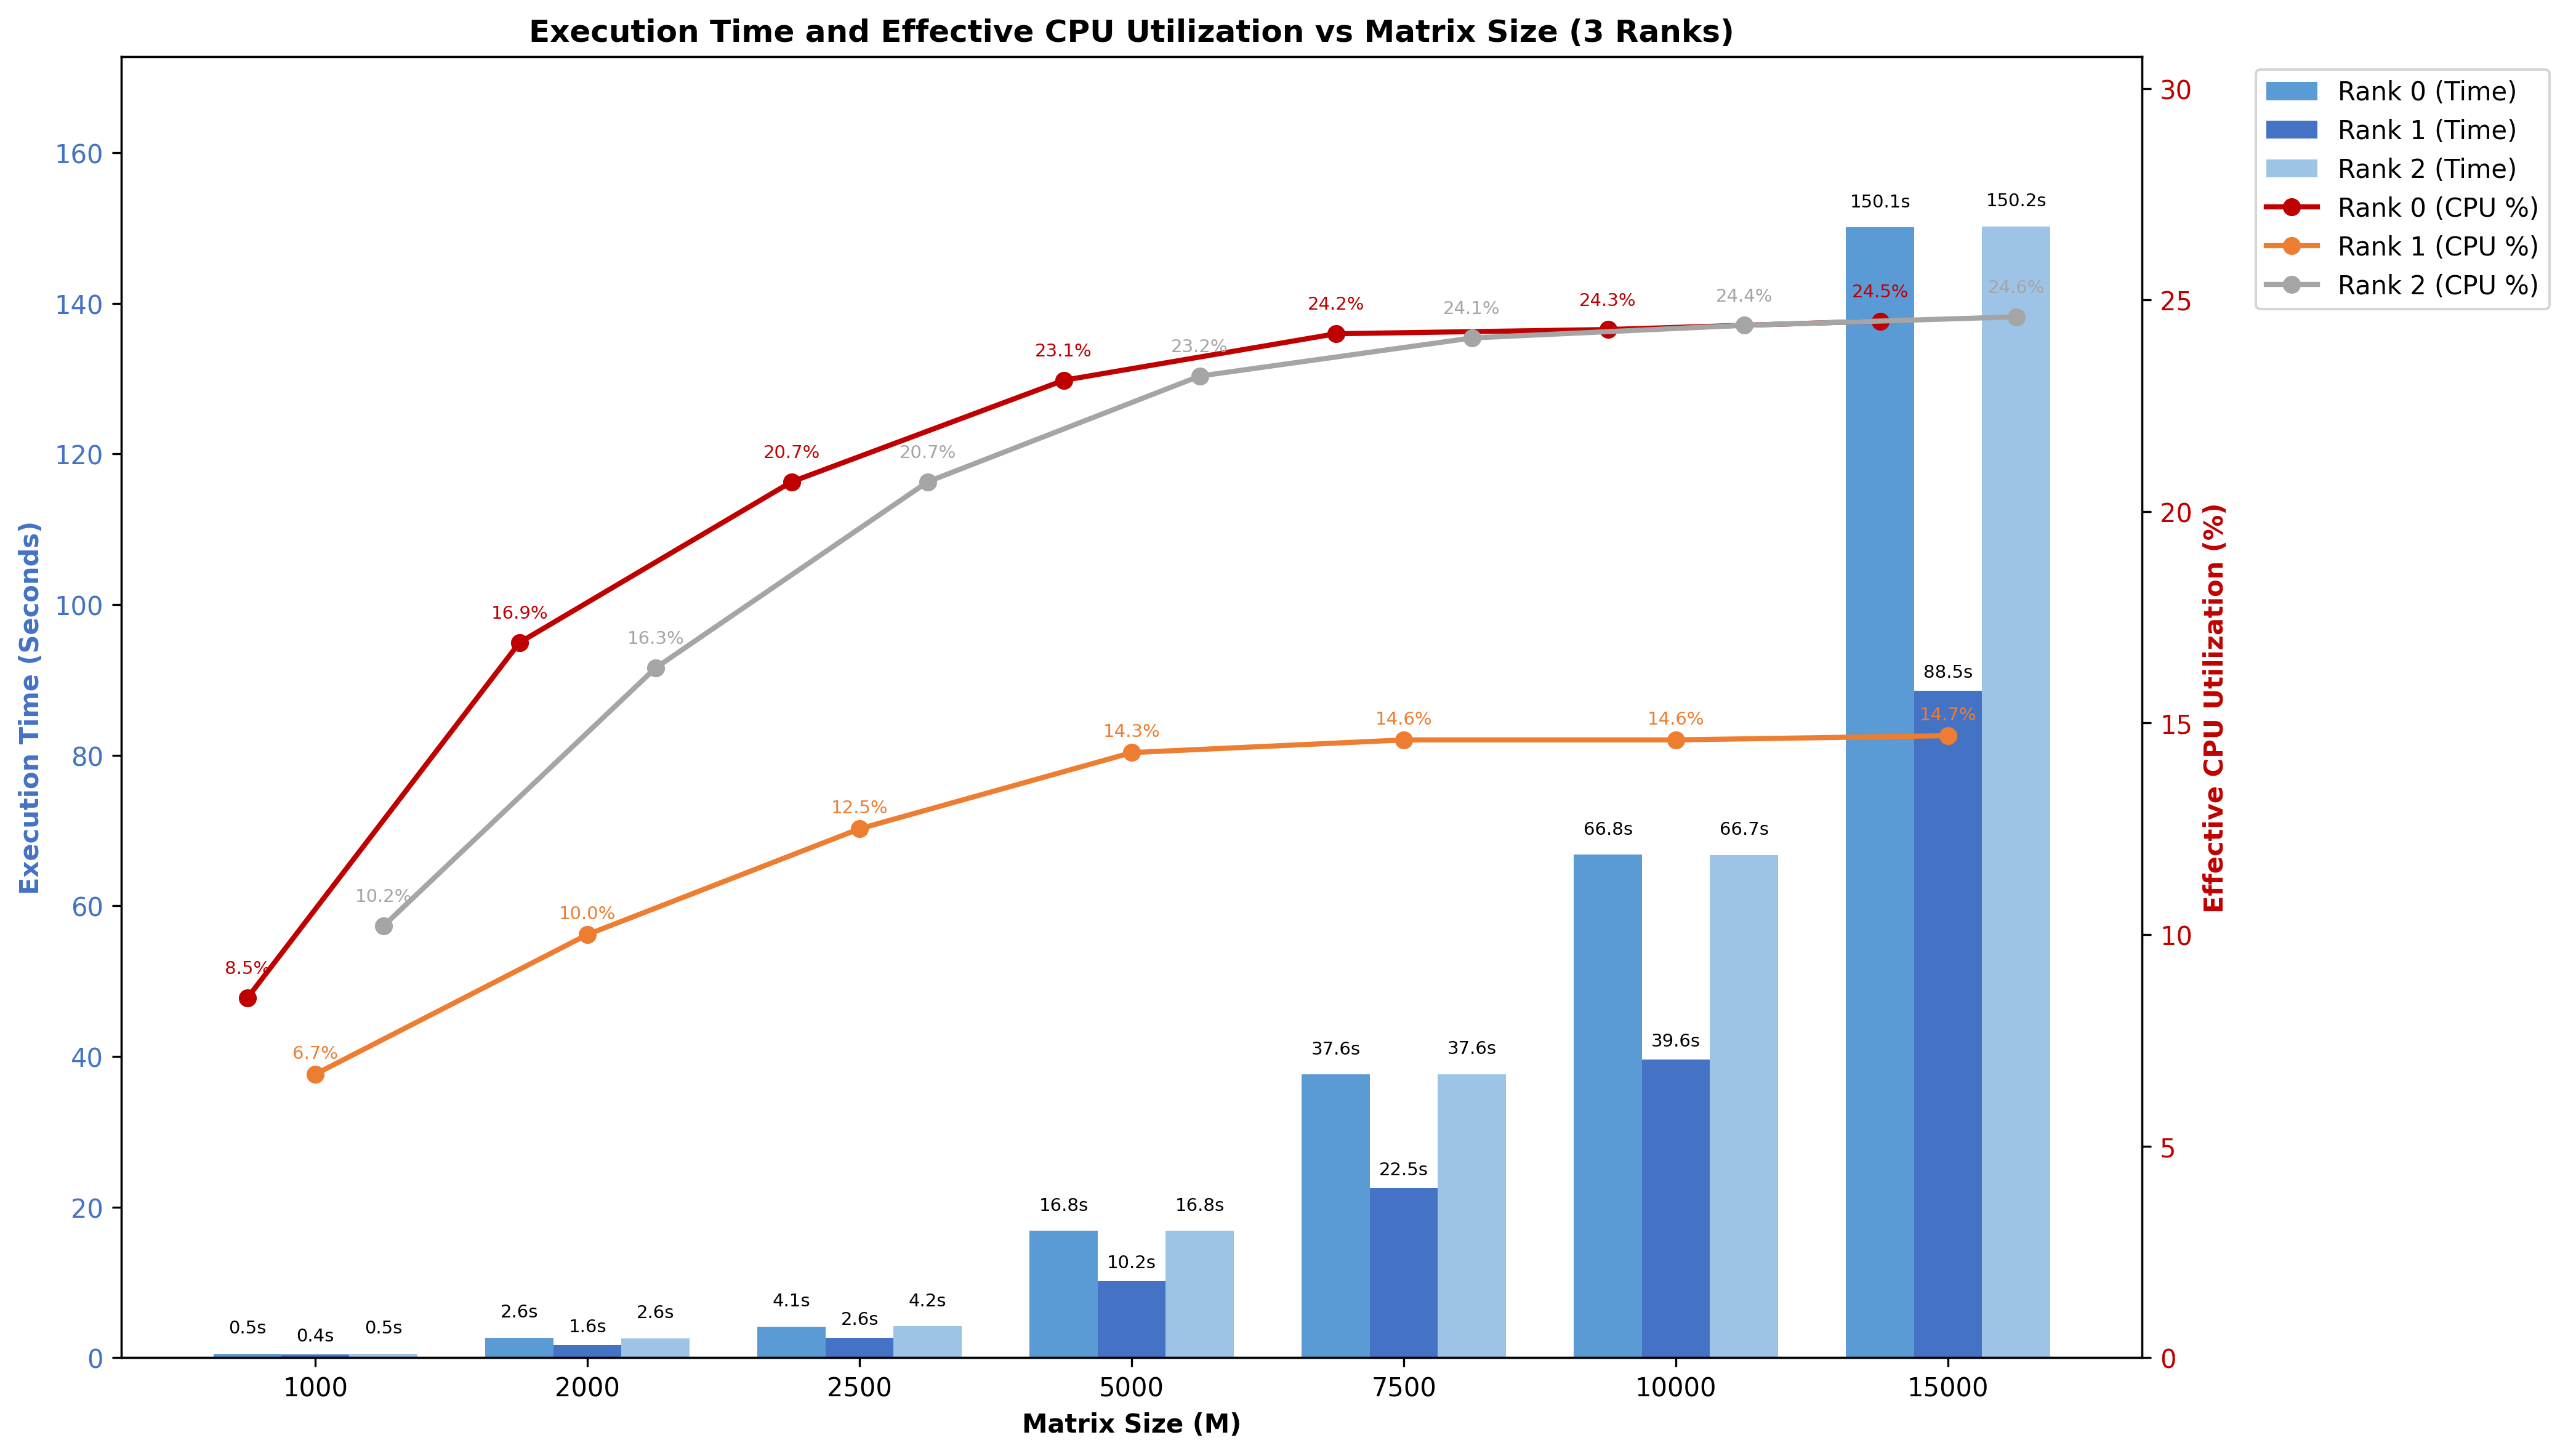
\includegraphics[width=0.9\textwidth]{../Giro_part/Esercizio_2/Grafici/combo_bars_lines_2socket.png}
    \caption{Execution Time and Effective CPU Utilization vs Matrix Size (Rank 1 isolated on a separate socket).}
    \label{fig:graph_isolated_socket}
\end{figure}

The results in Figure \ref{fig:graph_isolated_socket} perfectly illustrate the critical impact of memory bandwidth. By isolating Rank 1 on a separate socket, it gained unhindered access to the memory controller, allowing it to finalize its local stencil computations significantly faster than the other two processes, which were still competing for cache and RAM bandwidth on Socket 0 (e.g., executing in roughly 88 seconds versus 150 seconds).

However, this topology introduces a counter-intuitive phenomenon regarding the recorded CPU efficiency, caused by the global synchronization barrier. Because the overall application relies on \texttt{MPI\_Finalize} to terminate safely, Rank 1 completes its physical calculations early and subsequently enters a prolonged idle spin-wait state, waiting for Ranks 0 and 2 to finish. Since VTune averages the Effective CPU Utilization over the entire lifespan of the process, this extended idle period drastically dilutes Rank 1's final metric. This apparent efficiency degradation is, in reality, a direct proof of its superior execution speed: hardware isolation allowed the rank to severely outpace the others, trading measured CPU utilization for raw computational velocity.
